\section{信息的存储}
\subsection{使用比特表示信息}
\subsubsection{万物皆比特}
由于信号易存储在双稳态单元中,并且可以在存在噪声和不准确的信道中可靠地传输。信息都可以使用二进制的编码进行表示,计算机通过二进制来发送指令,以及表示和处理各种数字、字符串等。

\subsubsection{字节数据编码}
1 Byte = 8 bits。二进制表示范围是 \(00000000_{2}\) 到 \(11111111_{2}\);十进制表示范围是 \(0_{10}\) 到 \(255_{10}\);十六进制表示范围是 \(00_{16}\) 到 \(FF_{16}\),十六进制以 16 为基数,计数符号为 0 - 9 和 A - F 。在 C 语言中,FA1D37B$_{16}$ 可表示为 0xFA1D37B 或 0xfa1d37b。
\begin{table}[H]
    \captionsetup{skip=4pt}
    \centering
    \setlength{\arrayrulewidth}{1pt}
    \begin{tabular}{ccc}
        \hline
        \makebox[0.2\textwidth][c]{十进制} & \makebox[0.2\textwidth][c]{十六进制} & \makebox[0.2\textwidth][c]{二进制} \\
        \noalign{\global\setlength{\arrayrulewidth}{0.5pt}}
        \hline
        0                               & 00                               & 00000000                        \\
        1                               & 01                               & 00000001                        \\
        2                               & 02                               & 00000010                        \\
        3                               & 03                               & 00000011                        \\
        4                               & 04                               & 00000100                        \\
        5                               & 05                               & 00000101                        \\
        6                               & 06                               & 00000110                        \\
        7                               & 07                               & 00000111                        \\
        8                               & 08                               & 00001000                        \\
        9                               & 09                               & 00001001                        \\
        10                              & 0A                               & 00001010                        \\
        11                              & 0B                               & 00001011                        \\
        12                              & 0C                               & 00001100                        \\
        13                              & 0D                               & 00001101                        \\
        14                              & 0E                               & 00001110                        \\
        15                              & 0F                               & 00001111                        \\
        \noalign{\global\setlength{\arrayrulewidth}{1pt}}
        \hline
    \end{tabular}
    \caption{字节数据编码对应表}
\end{table}
\subsection{位运算}
\subsubsection{布尔代数}
\begin{itemize}
    \item And(与):\(A \& B = 1\) 当且仅当 \(A = 1\) 且 \(B = 1\)。
    \item Or(或):\(A | B = 1\) 当 \(A = 1\) 或者 \(B = 1\)。
    \item Not(非):\(\sim A = 1\) 当 \(A = 0\)。
    \item Exclusive - Or(Xor,异或):\(A\^{}B = 1\) 当 \(A = 1\) 或者 \(B = 1\),但不同时为 1,即相同为 0,不同为 1。
\end{itemize}

\subsubsection{C 语言中的位运算}
C 语言定义了四个位运算符号:
\begin{table}[H]
    \captionsetup{skip=4pt}
    \centering
    \setlength{\arrayrulewidth}{1pt}
    \begin{tabular}{cccc}
        \hline
        \makebox[0.15\textwidth][c]{C 表达式} & \makebox[0.2\textwidth][c]{二进制表达式} & \makebox[0.2\textwidth][c]{二进制结果} & \makebox[0.15\textwidth][c]{十六进制结果} \\
        \noalign{\global\setlength{\arrayrulewidth}{0.5pt}}
        \hline
        $\sim$ 0x41                        & $\sim$[0100 0001]                  & \([10111110]\)                    & 0xBE                                \\
        $\sim $ 0x00                       & \(\sim[0000 0000]\)                & \([11111111]\)                    & 0xFF                                \\
        0x69\&0x55                         & \([0110 1001]\&[0101 0101]\)       & \([0100 0001]\)                   & 0x41                                \\
        0x69 | 0x55                        & \([0110 1001] | [0101 0101]\)      & \([01111101]\)                    & 0x7D                                \\
        \noalign{\global\setlength{\arrayrulewidth}{1pt}}
        \hline
    \end{tabular}
    \caption{C 语言位运算示例}
\end{table}
\subsubsection{异或运算的应用:数据交换}
在 C 语言中,可以利用异或运算实现不使用额外变量交换两个数:
\begin{minted}{c}
void funny(int *x, int *y)
{
    *x = *x ^ *y; /* #1 */
    *y = *x ^ *y; /* #2 */
    *x = *x ^ *y; /* #3 */
}
\end{minted}
交换过程如下:
\begin{table}[H]
    \captionsetup{skip=4pt}
    \centering
    \setlength{\arrayrulewidth}{1pt}
    \begin{tabular}{ccc}
        \hline
        \makebox[0.1\textwidth][c]{步骤} & \makebox[0.2\textwidth][c]{*x}                     & \makebox[0.2\textwidth][c]{*y}     \\
        \noalign{\global\setlength{\arrayrulewidth}{0.5pt}}
        \hline
        开始                             & A                                                  & B                                  \\
        1                              & A\^{}B                                             & B                                  \\
        2                              & A\^{}B                                             & (A\^{}B)\^{}B = A\^{}(B\^{}B) =  A \\
        3                              & (A\^{}B)\^{}A = (B\^{}A)\^{}A = B\^{}(A\^{}A)  = B & A                                  \\
        结束                             & B                                                  & A                                  \\
        \noalign{\global\setlength{\arrayrulewidth}{1pt}}
        \hline
    \end{tabular}
    \caption{异或运算交换数据过程}
\end{table}
\subsubsection{C 语言中的逻辑运算}
C 语言定义了三种逻辑运算:\(||\)(逻辑或)、\&\&(逻辑与)、\(!\)(逻辑非),具有短路效应。例如:
\begin{itemize}
    \item x \&\& 5/x 可以用于避免除 0 运算。
    \item p \&\& *p++ 可以避免空指针运算。
    \item 5 || x = y 赋值语句将不会被执行。
\end{itemize}
\subsubsection{C 语言中的移位运算}
C 语言中有逻辑移位和算术移位。右移运算有逻辑移位(左侧补 0)和算术移位(左侧补原最高位值)两种操作。对于无符号数,右移是逻辑的;对于有符号数,几乎所有的编译器针对有符号数的右移都采用的是算术右移
\begin{figure}[H]
    \centering
    \captionsetup{skip=4pt}
    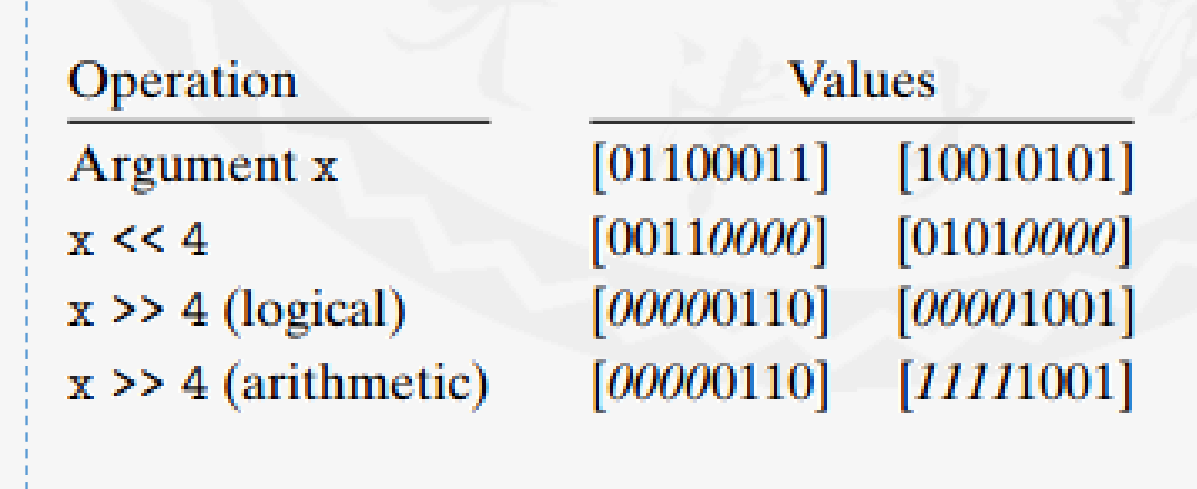
\includegraphics[width=6cm]{3.png}
    \caption{移位运算}
\end{figure}
\subsubsection{未定义行为}
C 语言规范中没有被明确定义的行为称为未定义行为(UB),编程时应避免使用未定义行为,但有符号数算术右移除外。例如,移位 \(k\),当 \(k\) 大于等于变量位长时,值直接变为0,在 GCC 中的实现如下:
\begin{minted}{c}
int aval = 0x0EDCBA98 >> 36; 
movl $0, -8(%ebp)   // 值直接变为0
unsigned uval = 0xFEDCBA98u << 40;
movl $0, -4(%ebp)   // 值直接变为0
\end{minted}
\subsubsection{运算优先级}
移位运算符的优先级低于加减乘除,例如 \(- 1<<2+3<<4\),正确的运算顺序为 \((1<<(2 + 3))<<4\) 。
\subsection{信息的存储和表示}
\subsubsection{字长}
字长是指针数据的大小(虚拟地址宽度)。 32 位 ( 4 字节) 计算机字长限制了地址空间为 4GiB(\(2^{32}\) 字节);64 位字长( 8 字节)寻址能力达到了 18EiB
\subsubsection{C 语言中的各数据类型位宽}
计算机和编译器支持多种数据类型,或是小于字长,或大于字长,但长度都是整数个字节。
\begin{table}[H]
    \captionsetup{skip=4pt}
    \centering
    \setlength{\arrayrulewidth}{1pt}
    \begin{tabular}{cccc}
        \hline
        \makebox[0.15\textwidth][c]{数据类型} & \makebox[0.15\textwidth][c]{32 位系统} & \makebox[0.15\textwidth][c]{64 位系统} & \makebox[0.15\textwidth][c]{x86 - 64} \\
        \noalign{\global\setlength{\arrayrulewidth}{0.5pt}}
        \hline
        char                                  & 1                                      & 1                                      & 1                                     \\
        short                                 & 2                                      & 2                                      & 2                                     \\
        int                                   & 4                                      & 4                                      & 4                                     \\
        long                                  & 4                                      & 8                                      & 8                                     \\
        float                                 & 4                                      & 4                                      & 4                                     \\
        double                                & 8                                      & 8                                      & 8                                     \\
        pointer                               & 4                                      & 8                                      & 8                                     \\
        \noalign{\global\setlength{\arrayrulewidth}{1pt}}
        \hline
    \end{tabular}
    \caption{C 语言数据类型位宽}
\end{table}
\subsubsection{字节序}
有小端序(Little endian)和大端序(Big endian)两种。小端序低地址存放低位数据,高地址存放高位数据;大端序低地址存放高位数据,高地址存放低位数据。例如,对于 0x1234567 :
\begin{figure}[H]
    \centering
    \captionsetup{skip=4pt}
    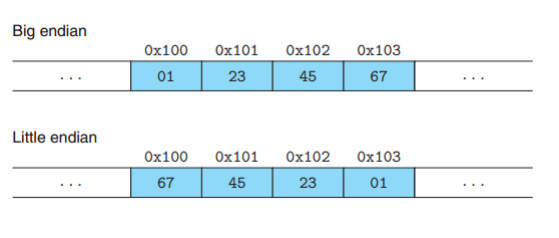
\includegraphics[width=10cm]{7.png}
    \caption{小端序和大端序} 
\end{figure}

\subsubsection{探索数据在存储器中的存储方式}
通过以下代码可以打印各变量的字节表示形式:
\begin{minted}{c}
#include <stdio.h>
typedef unsigned char *byte_pointer;    //unsigned char占用一个字节,可以做到逐字节访问内存
void show_bytes(byte_pointer start,int len){
    int i;
    for(i = 0; i < len; i++)
        printf("%.2x ",start[i]);
    printf("\n");
}
void show_int(int x){
    show_bytes((byte_pointer)&x, sizeof(int));
}
void show_float(float x){
    show_bytes((byte_pointer)&x, sizeof(float));
}
void show_pointer(void *x){
    show_bytes((byte_pointer)x, sizeof(void*));
}
\end{minted}
在 Linux32/64(小端)、Win32(小端)和 Sun(32 位,大端)系统下的测试数字 12345 (0x00003039)结果如下。对于指针的存储,不同的编译器和计算机可能会分配不同的地址,甚至每一次运行时得到的结果都不相同。
\begin{table}[H]
    \captionsetup{skip=4pt}
    \centering
    \setlength{\arrayrulewidth}{1pt}
    \begin{tabular}{cccc}
        \hline
        \makebox[0.1\textwidth][c]{机器} & \makebox[0.1\textwidth][c]{值}           & \makebox[0.1\textwidth][c]{类型} & \makebox[0.2\textwidth][c]{字节(从左到右地址升高)} \\
        \noalign{\global\setlength{\arrayrulewidth}{0.5pt}}
        \hline
        Linux 32                       & 12345                                   & int                            & 39 30 00 00                          \\
        Windows                        & 12345                                   & int                            & 39 30 00 00                          \\
        Sun                            & 12345                                   & int                            & 00 00 30 39                          \\
        Linux 64                       & 12345                                   & int                            & 39 30 00 00                          \\
        Linux 32                       & 12345.0                                 & float                          & 00 e4 40 46                          \\
        Windows                        & 12345.0                                 & float                          & 00 e4 40 46                          \\
        Sun                            & 12345.0                                 & float                          & 46 40 e4 00                          \\
        Linux 64                       & 12345.0                                 & float                          & 00 e4 40 46                          \\
        Linux 32                       &       \& ival                       & int *                          & e4 f9 ff bf                          \\
        Windows                        &                             \& ival & int *                          & b4 cc 22 00                          \\
        Sun                            &                             \& ival & int *                          & ef ff fa 0c                          \\
        Linux 64                       &                             \& ival & int *                          & b8 11 e5 ff ff 7f 00 00              \\
        \noalign{\global\setlength{\arrayrulewidth}{1pt}}
        \hline
    \end{tabular}
    \caption{不同系统下数据存储测试结果}
\end{table}

\subsubsection{字符串的表示}
C 语言的字符串使用 char 数组表示,每个字符都被编码成 ASCII 码,是一个 7 比特的字符编码集(扩展集为 8 比特)。字符“0”的编码是 0x30,数字字符 \(i\) 的编码是 0x30 \(+ i\) 。字符串的结尾应为空字符,即 ASCII 编码为 0 。字符串的表示与字节序无关,大小端兼容,因为每个 char 只占用一个字节,单独存储时和大小端无关

\subsubsection{小知识:PE 和 ELF 格式}
Windows 操作系统下常用的可执行文件格式是 PE(Portable Executable);Unix 家族(含 Linux)操作系统下可执行文件格式为 ELF(Executable and Linkable Format)。
